%\documentclass[14pt, notes]{beamer}
\documentclass[14pt]{beamer}

%\usepackage{pgfpages}
%\setbeameroption{show notes}
%\setbeameroption{show notes on second screen=right}

%encoding
\usepackage[utf8]{inputenc}

%language
\usepackage[russian]{babel}
\usepackage{amsmath}
\usepackage{bm}
\usepackage{graphicx}
\usepackage{hyperref}
\graphicspath{{images/}}%путь к рисункам

\setbeamerfont{author in head/foot}{size=\small}
\setbeamerfont{title in head/foot}{size=\footnotesize}

\title{Метод погруженной границы}
\date{\today}
\author{Долгов Д.А.}
\institute{Кемеровский Государственный Университет \\
    \vspace{0.7cm}
    \vspace{0.7cm}
} 
\usetheme[numbers, totalnumbers, minimal, nologo]{Statmod}
% Привычный шрифт для математических формул
\usefonttheme[onlymath]{serif}

\definecolor{statmodblue}{RGB}{100,10,30}
\definecolor{statmodsand}{RGB}{244,215,103}

\begin{document}
\maketitle

%description of the problem
\begin{frame}
\frametitle{Описание задачи}
\begin{itemize}
	\item Клапан - часть сердца, образованная складками его внутренней оболочки (лепестками), обеспечивает однонаправленный ток крови.
	\item Для замены поврежденных могут использоваться искусственные клапаны, к которым предъявляется множество требований.
\end{itemize}
\end{frame}
\note{Для оценки - каждый год проводится примерно 250 000 по восстановлению или замене поврежденных сердечных клапанов}

%description of the problem: topicality
\begin{frame}
\frametitle{Введение}
\setbeamercolor{normal text}{fg=gray,bg=}
\setbeamercolor{alerted text}{fg=black,bg=}
\usebeamercolor{normal text}
\begin{itemize}
    \item \alert<+>{Механизмы ряда явлений, например, нелинейного искажения формы пульсовых волн, изучены недостаточно}
    \item \alert<+>{Существует прямая связь между гидродинамическими параметрами и развитием патологический изменений в сосудистых стенках, клапанах и т.д.}
    \item \alert<+>{Развитие различных методов измерения на моделях и в организмах позволяет выявить многочисленные детали, требующие объяснения}
\end{itemize}
\end{frame}

%description of the problem: topicality
\begin{frame}
\frametitle{Введение}
\begin{itemize}
	\item Создание клапанов требует решения большого количества задач (уменьшение тромбогенезиса, износа, градиента давления, увеличение безопасности и т.д.).
    \item Частично эти задачи можно решить с помощью математического моделирования
\end{itemize}
\end{frame}

%complexity with image
\begin{frame}
\frametitle{Построения расчетной области}
    \begin{center}
        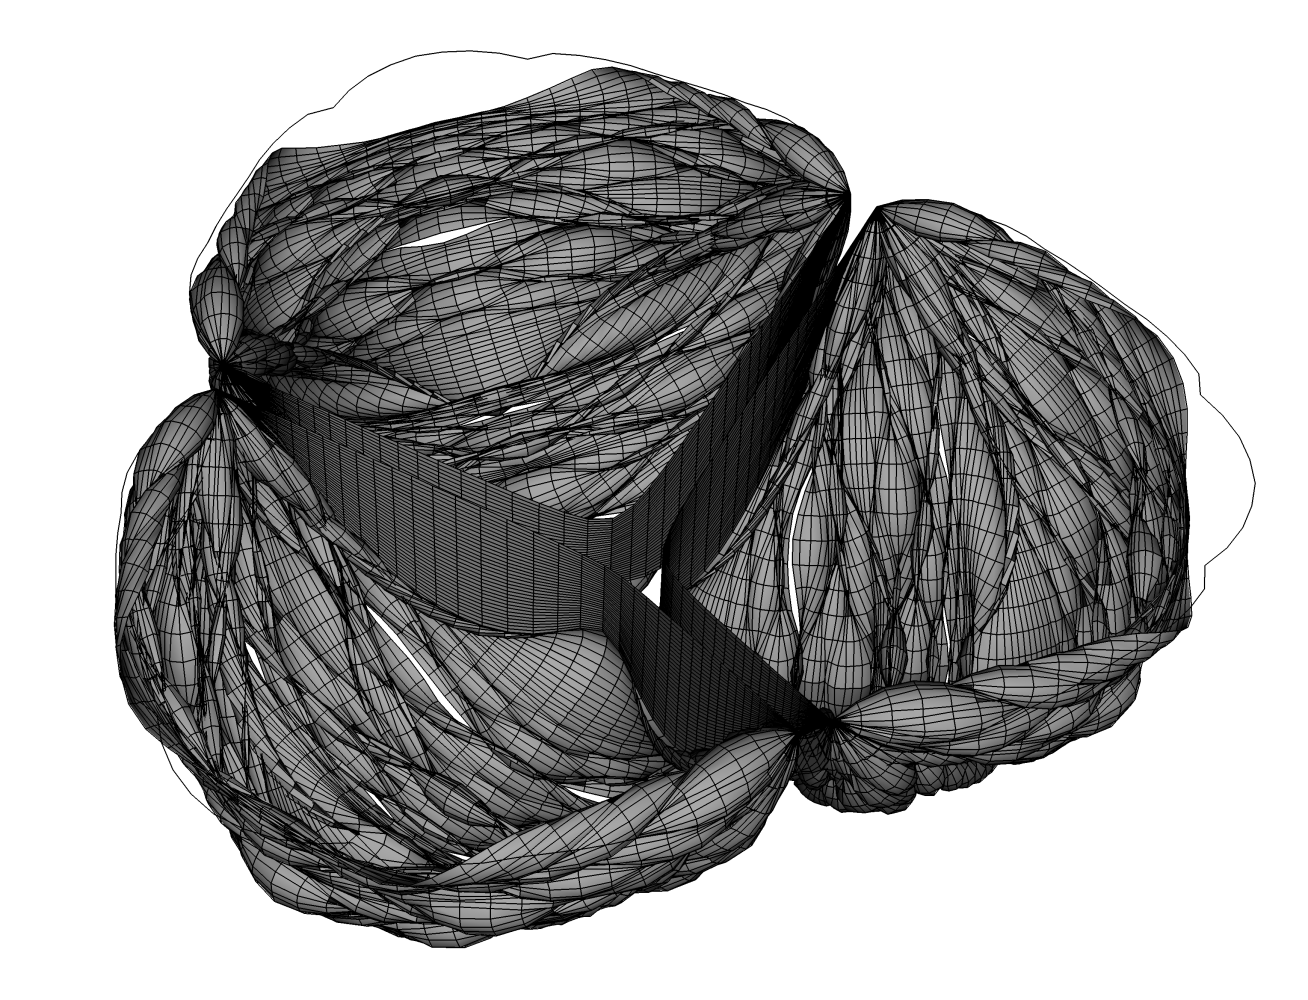
\includegraphics[width=9cm]{immersed_boundary/aortic_valve_mesh.png}
    \end{center}
\end{frame}
\note{Пример достаточно сложной модели клапана}

%possible solution method
\begin{frame}
\frametitle{Существующие методы}
\setbeamercolor{normal text}{fg=gray,bg=}
\setbeamercolor{alerted text}{fg=black,bg=}
\usebeamercolor{normal text}
\begin{itemize}
    \item \alert<+>{Метод адаптивных сеток}
    \item \alert<+>{Метод конечных элементов}
    \item \alert<+>{Метод погруженной границы}
\end{itemize}
\end{frame}
\note{Первые два будут рассмотрены обзорно, последний описан более подробно. Я собираюсь использовать его в работе, т.к. в теории он потребует наименьшей переделки текущей реализации программы}

%adaptive mesh refinement
\begin{frame}
\frametitle{Метод адаптивных сеток}
    \begin{center}
        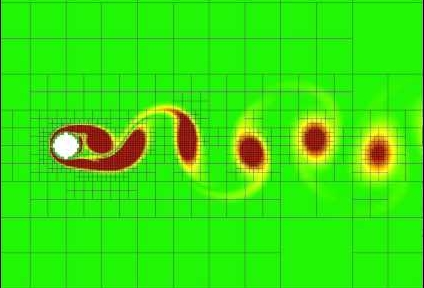
\includegraphics[width=9cm]{immersed_boundary/adaptive_mesh.jpg}
    \end{center}
\end{frame}
\note{Суть метода заключается в построении таких сеток, которые будут хорошо согласованы с расчетной областью и получаемым решением по каким-либо параметрам}

%adaptive mesh refinement
\begin{frame}
\frametitle{Метод адаптивных сеток}
\setbeamercolor{normal text}{fg=gray,bg=}
\setbeamercolor{alerted text}{fg=black,bg=}
\usebeamercolor{normal text}
\begin{itemize}
    \item \alert<+>{Геометрические адаптивные сетки\\ (Подстраиваются под границы)}
    \item \alert<+>{Динамические адаптивные сетки\\ (Подстраиваются под решение)}
\end{itemize}
\end{frame}
\note{Геометрические - адаптируются к границам расчетной области, динамические - к получаемому решению, т.е. эти сетки могут <<сгущаться>> в нужных местах. Помимо этих свойств, подобные методы характеризуются множеством других особенностей - добавляются ли новые узлы или только перемещаются имеющиеся, сохраняется ли структурированность сетки или нет. Естесственно, существует также множество алгоритмов адаптации, например таковой, где ребра сетки приравниваются к пружинам с жесткостью, зависящей от свойств среды. Но я не буду на этом особо останавливаться, это тема для отдельного большого разговора.}

%snappyHexMesh
\begin{frame}
    \frametitle{SnappyHexMesh utility (OpenFOAM)}
    \begin{center}
        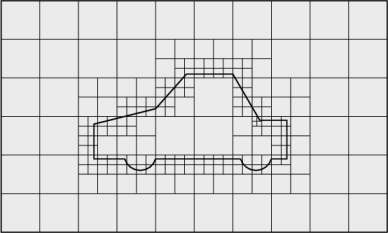
\includegraphics[width=7cm]{immersed_boundary/snappy.png}
    \end{center}
    В формате STL описывается поверхность границы, затем создается предварительная сетка, которая улучшается в несколько этапов.
\end{frame}
\note{В заключении рассказа об адаптивных сетках замечу, что уже существуют достаточно хорошие <<пакетные>> реализации подобных механизмов. Один из них - утилита SnappyHexMesh, входящая в состав пакета OpenFOAM. На слайде приведен пример получения адаптивной сетки с его помощью}

%finite element 
\begin{frame}
\frametitle{Метод конечных элементов}
    \begin{center}
        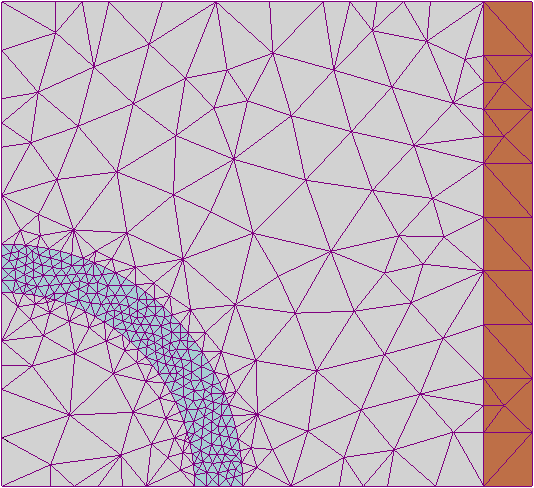
\includegraphics[width=5cm]{immersed_boundary/Example_of_2D_mesh.png}
    \end{center}
    Сетки, используемые в МКЭ позволяют легко представить нужную область.
\end{frame}
\note{Т.к. в МКЭ дискретизация области происходит с помощью локальных элементов (например, треугольников) - это позволяет легко смоделировать в расчете нужную геометрию области}

%finite element 
\begin{frame}
    \frametitle{Метод конечных элементов (3D)}
    \begin{center}
        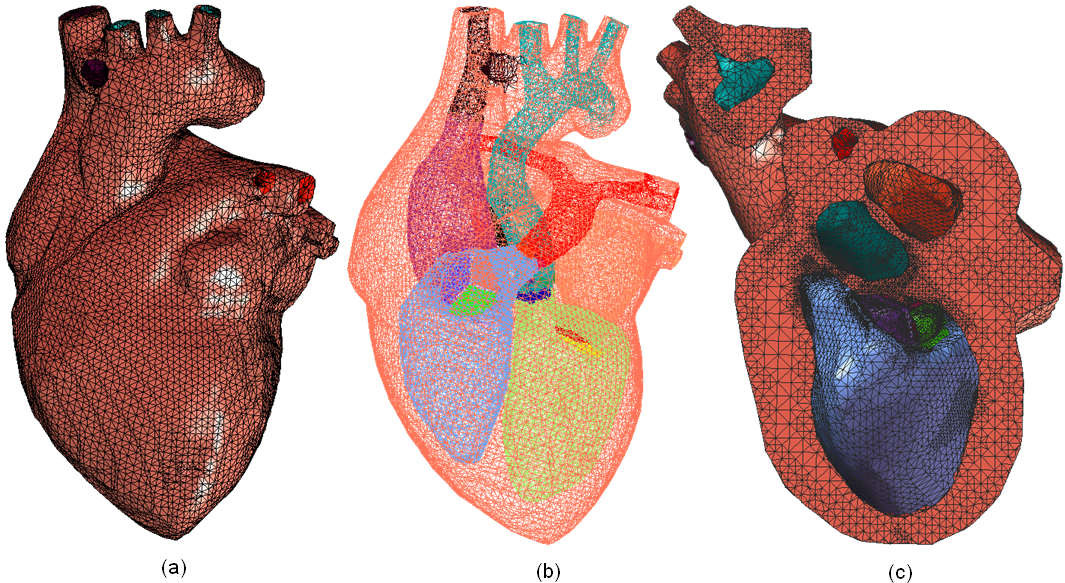
\includegraphics[width=10cm]{immersed_boundary/heart_bound.png}
    \end{center}
\end{frame}
\note{В случае 3х измерений дискретизация становится не такой очевидной, но тем не менее возможна. Опять же, не буду долго задерживаться на описании этого метода}

%immersed boundary 
\begin{frame}
\frametitle{Метод погруженной границы}
Метод позволяет моделировать взаимодействие жидкости и погруженных в нее структур. Исходная версия была опубликована в работе <<C.S. Peskin, Numerical Analysis of Blood Flow in the Heart, J. Comput. Phys. 25 (1977). Используется для моделирования биологических явлений.
\end{frame}

%immersed boundary 
\begin{frame}
\frametitle{Метод погруженной границы}
Основная идея заключается в проведении расчета на обычной декартовой сетке. Сложная форма исследуемого объекта учытывается не при построении сетки, а на других этапах.
\end{frame}

%immersed methods 
\begin{frame}
\frametitle{Вариации метода}
\setbeamercolor{normal text}{fg=gray,bg=}
\setbeamercolor{alerted text}{fg=black,bg=}
\usebeamercolor{normal text}
\begin{itemize}
    \item \alert<+>{Оригинальный метод, который предложил C.S. Peskin}
    \item \alert<+>{Метод <<фиктивных>> ячеек (ghost cells)}
    \item \alert<+>{Метод <<усеченных>> ячеек (cut cells)}
\end{itemize}
\end{frame}
\note{Сравнивать я буду в основном первые два, т.к. последний используется с методом конечных объемов и я не стал его рассматривать. В кратце - его основная идея в разбиении ячеек, через которые проходит погруженная граница, и дальшейшей интепроляции полученных значений}

%original method 
\begin{frame}
\frametitle{Метод погруженной границы}
В несжимаемую вязкую ньютоновскую жидкость помещены тонкие <<волокна>>, которыми могут моделироваться сердечные клапаны, мышцы или искусственные клапаны. Они двигаются под влиянием течения жидкости и сами влияют на нее.
Чтобы учесть влияние клапанов на течение, в уравнение Навье-Стокса вводится функция плотности силы $F(x, t)$
\begin{equation}
    \rho (\frac{\partial u}{\partial t} + u \cdot \nabla u) = - \nabla p + \nu \triangle u + F
\end{equation}
\end{frame}
\note{Используемые волокна состоят в конечном счете из безмассовых точек, которые движутся со скоростью жидкости и влияют на нее только посредством силы напряжения}

%original method 
\begin{frame}
\frametitle{Метод погруженной границы}
    \begin{center}
        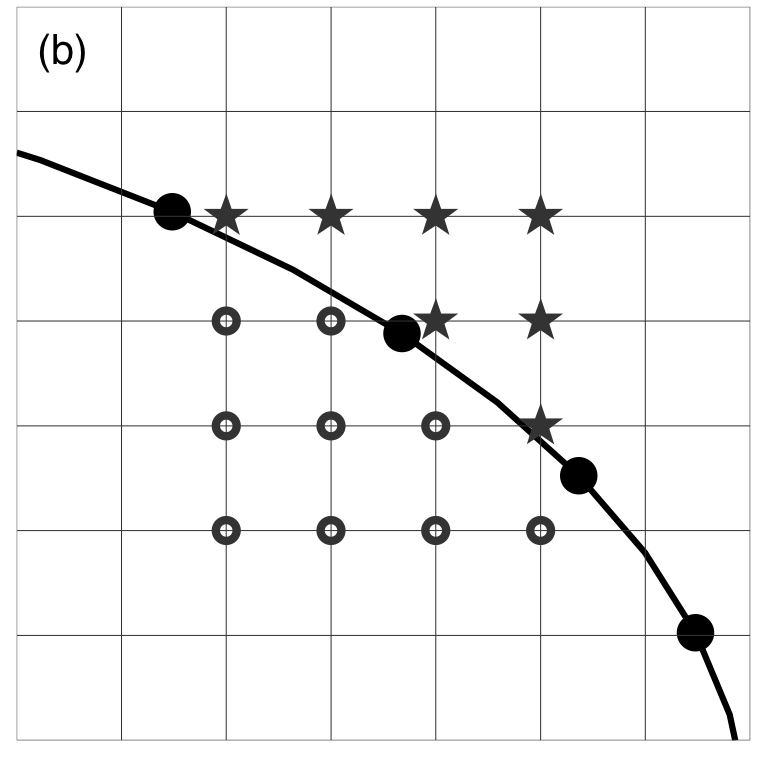
\includegraphics[width=7cm]{immersed_boundary/IBM_1b.jpg}
    \end{center}
\end{frame}
\note{На картинке изображена схема получающейся в итоге сетки - черные круги, не совпадающие с узлами сетки, представляют погруженную границу, которая разделяет жидкость и твердую поверхность}

%original method 
\begin{frame}
\frametitle{Метод погруженной границы}
Для расчета $F$, погруженная граница представляется в лагранжевых координатах

\begin{gather}
\label{eq:ib_motion}
\frac{d x_k}{d t} = u(x_k, t) = \int_{x \in \Omega} u(x, t) \delta(x-x_k) dv\\
\label{eq:force_density}
F(x) = \lim_{N \to \inf} (\frac{1}{N}) \sum_{k=1}^N f_k \delta(x-x_k)\\
f_k = f_k(x_1, x_2, \ldots)
\end{gather}
\end{frame}
\note{Т.к. для вычисления силы напряжения используются параметры, связанные с погруженной границей, они должны расчитываться в Лагранжевых координатах. На представленных формулх, $\delta$ - дельта функция дирака, которая при переходе к численному решению заменяется дискретным аналогом. $x_1, x_2, \ldots$ - координаты точек погруженной границы, $f_1, f_2, \ldots$ - сила напряжения в точке}

%original method 
\begin{frame}
\frametitle{Метод погруженной границы}
Для двух точек границы $A$, $B$, где $T$ - напряжение связи между точками.

\begin{gather}
\label{eq:link_struct}
L_{AB} = \| x_B - x_A \| \\
\frac{1}{N}f_A = \sum_{B=1; B \neq A}^{N} T_{AB}(L_{AB})\frac{x_B-x_A}{\| L_{AB} \|}
\end{gather}
\end{frame}
\note{В простейшем случае, погруженная граница моделируется набором точек и связей между ними}

%original method 
\begin{frame}
\frametitle{Метод погруженной границы}
В двумерном случае для сердечного клапана

\begin{gather}
\label{eq:valve_leaflet}
T(L)=(L-L_0)S, \; L > L_0 \\
T(L)=0, \; L \leq L_0,
\end{gather}
где $S$ - коэффициент жесткости, $L_0$ - остаток длинны клапана
\end{frame}
\note{В статьях, посвященных этому методу, разработано несколько способов моделировать различные ситуации - естесственные аортальные, митральные клапаны, сердечные мышцы, искусственные клапаны.}

%original method 
\begin{frame}
\frametitle{Связь границы и жидкости}
Т.к. точки на погруженной границе не совпадают с точками жидкости, возникает необходимость интерполяции скорости на границу и распределение плотности силы на точки жидкости

\begin{gather}
\label{eq:interpolation}
u_k = \sum_{ij}h^{2} u_{ij} D_{ij}(x_k) \\
\label{eq:spreading}
F_{ij} = \frac{1}{N} \sum_k f_k D_{ij}(x_k)
\end{gather}

$D_{ij}(x_k)$ соответствует $\delta(x-x_k)$
\end{frame}

%original method 
\begin{frame}
\frametitle{Связь границы и жидкости}
Для $\bm x=(x, y)$
\begin{gather}
\label{eq:force}
D_{ij}(\bm x) = d(x-ih)(y-jh) \\
\label{eq:delta_function}
d(r) = \frac{1}{4h}(1 + cos(\frac{\pi r}{2h})), \; \|r\| < 2h \\
d(r) = 0, \; \|r\| \geq 2h
\end{gather}
\end{frame}

%original method 
\begin{frame}
\frametitle{Связь границы и жидкости}
    \begin{center}
        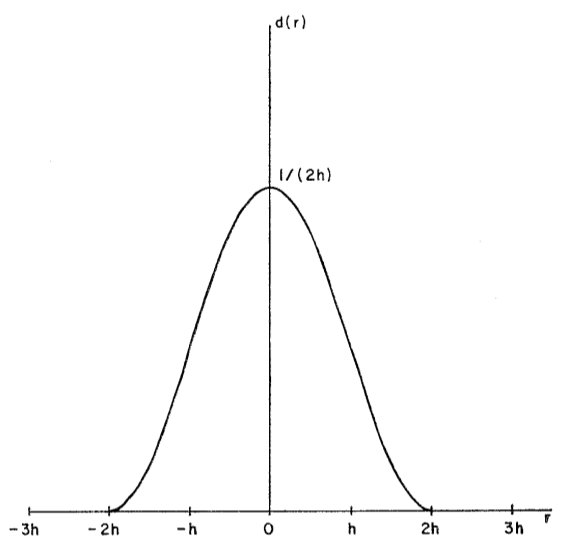
\includegraphics[width=7cm]{immersed_boundary/delta_function.png}
    \end{center}
\end{frame}
\note{Выбор дискретного представления дельта функции - один из ключевых моментов метода, было предложено несколько вариантов. Основная проблема в данном случае, чтобы дельта функция удовлетворяла определенным условиям, которые требуются для сходимости метода.}

%original method 
\begin{frame}
\frametitle{Твердые границы}
Описанный подход хорошо подходит для моделирования гибких границ, в то время как для жестких приходится использовать его различные модификации.
\end{frame}
\note{Опять же, эти модификации разнообразны, например, рассматривать погруженную границу, как гибкую с чрезвычайно большим коэффициентом жесткости}

%original method 
\begin{frame}
\frametitle{Алгоритм}
\setbeamercolor{normal text}{fg=gray,bg=}
\setbeamercolor{alerted text}{fg=black,bg=}
\usebeamercolor{normal text}
    \begin{itemize}
        \item \alert<+>{Вычисление во всех точках силы $f(x_1, x_2, \ldots)$ на основе деформации границы}
        \item \alert<+>{Распределение сил на узлы решетки и получение плотности силы F(x, t)}
        \item \alert<+>{Используя какой-либо метод, произвести расчет нового состояния жидкости с учетом F}
        \item \alert<+>{С помощью полученной скорости жидкости вычислить скорость движения точек границы}
        \item \alert<+>{Получение лагранжевых координат точек границы}
    \end{itemize}
\end{frame}

%ghost-cells method 
\begin{frame}
\frametitle{Метод <<фиктивных>> ячеек}
Альтернативный подход, в котором погруженная граница учитывается на этапе дискретизации с помощью <<фиктивных>> ячеек.
Для каждой из таких ячеек используется интерполяционная схема, которая неявно учитывает условия на погруженной границе.
\end{frame}
\note{Фиктивной называется узел, относящийся к твердой поверхности и имеющий как минимум одну соседную точку, относящуюся к жидкости}

%ghost-cells method 
\begin{frame}
\frametitle{Метод <<фиктивных>> ячеек}
    \begin{center}
        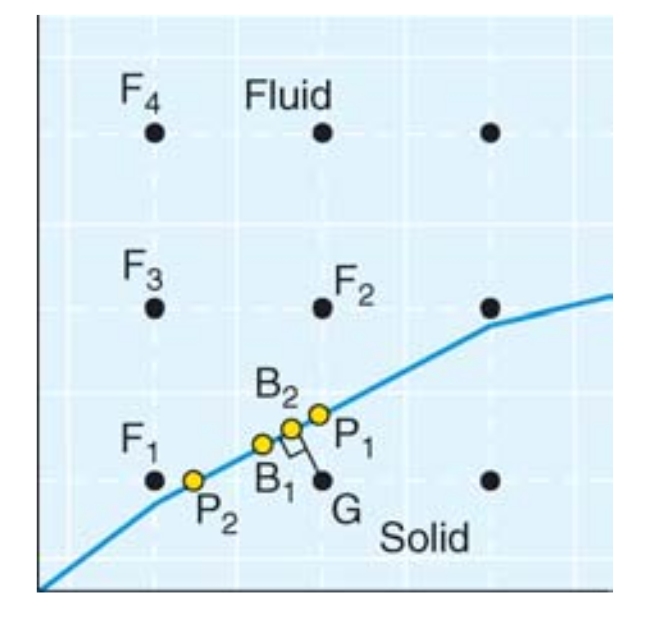
\includegraphics[width=7cm]{immersed_boundary/ghost-cells.png}
    \end{center}
\end{frame}
\note{На картинке схематично изображены действующие лица данного метода. В данном случае т. G будет являться <<фиктивной>>, поэтому значение в этой точке вычисляеся с помощью интерполяции точек $F_1, F_2, F_3$ (в линейном случае можно обойтись первыми двумя) и одной из точек на границе - $B_1, B_2$ (первая взята перпендикуляром, вторая - середина $P_1, P_2$). $P_1, P_2$ образованы пересечением границы с сеткой}

%ghost-cells method 
\begin{frame}
\frametitle{Метод <<фиктивных>> ячеек}
В простейшем случае используется билинейная (трилинейная для 3D) интерполяция
\begin{gather}
\label{eq:ghost_cell_iterpolation}
\phi = C_1 x_1 x_2 + C_2 x_1 + C_3 x_2 + C_4,
\end{gather}
где коэффициенты выражаются с помощью 3-х точек жидкости и одной точки на погруженной границе.
\end{frame}
\note{Здесь $\phi$ - значение некоторой переменной (например, скорость) в фиктивной ячейке, коэффициенты $C_i$ определяются из значений этой переменной в окружающих точках жидкости. Нахождение коэффициентов $C$ сводится к решению слау с матрицей Вандермонда. Зачастую, для избежания некоторых негативных счетных эффектов, сначала вычисляют значение в точке, которая является образом, а затем в самой фиктивной ячейке.}


%ghost-cells method 
\begin{frame}
\frametitle{Метод <<фиктивных>> ячеек}
Подобная интерполяция хорошо подходит для ламинарных течений и для некоторых течений с высокими числами Рейнольдса.
Для других случаев может быть использована интерполяция более высоких порядков. 
\end{frame}

%consideration
\begin{frame}
\frametitle{Недостатки}
\setbeamercolor{normal text}{fg=gray,bg=}
\setbeamercolor{alerted text}{fg=black,bg=}
\usebeamercolor{normal text}
    \begin{itemize}
        \item \alert<+>{<<Непрервыный>> подход вносит некоторые ограничения, связанные со сходимостью. Он не всегда подходит для расчетов с большими числами Рейнольдса, т.к. описывает <<смазанную границу>>
}
        \item \alert<+>{<<Дискретный>> подход обычно требует указания давления на погруженной границе и имеет некоторые сложности с моделированием движущихся погруженных границ.}
    \end{itemize}
\end{frame}

%ibamr: brief about source code
\begin{frame}
\frametitle{IBAMR}
\setbeamercolor{normal text}{fg=gray,bg=}
\setbeamercolor{alerted text}{fg=black,bg=}
\usebeamercolor{normal text}
    \begin{itemize}
        \item \alert<+>{PETSc, the Portable, Extensible Toolkit for Scientific Computation}
        \item \alert<+>{hypre, библиотека высокопроизводительных предобуславливателей}
        \item \alert<+>{HDF5, библиотека, реализцующая формат хранения научных данных HDF5}
        \item \alert<+>{Blitz++, высокопроизводительная библиотека для работы с массивами}
        \item \alert<+>{Silo, библиотека для работы с форматом визуализации и пост-обработки данных Silo}
    \end{itemize}
\end{frame}
\note{Основной вклад в разработку внесли сотрудники New York University School of Medicine. Библиотеки:

\begin{itemize}
    \item PETSc is funded primarily by the United States Department of Energy, Office of Science, by the Advanced Scientific Computing Research (ASCR) Applied Mathematics Research and SciDAC programs
    \item hypre - Center for Applied Scientific Computing
    \item The Blitz++ project started at the Vision and Image Processing Lab in the Dept. of Systems Design Engineering at the University of Waterloo (Canada)
\end{itemize}

Собирать из development ветки - ibamr-dev
}

%examples: aortic heart valve
\begin{frame}
\frametitle{Аортальный клапан}
    \begin{center}
	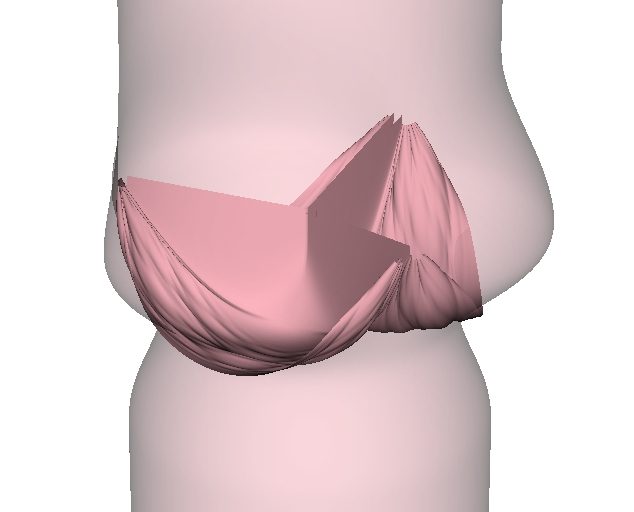
\includegraphics[width=8cm]{immersed_boundary/valve_vessel_side_crop.jpg}
    \end{center}
\end{frame}

\begin{frame}
\frametitle{Аортальный клапан}
    \begin{center}
	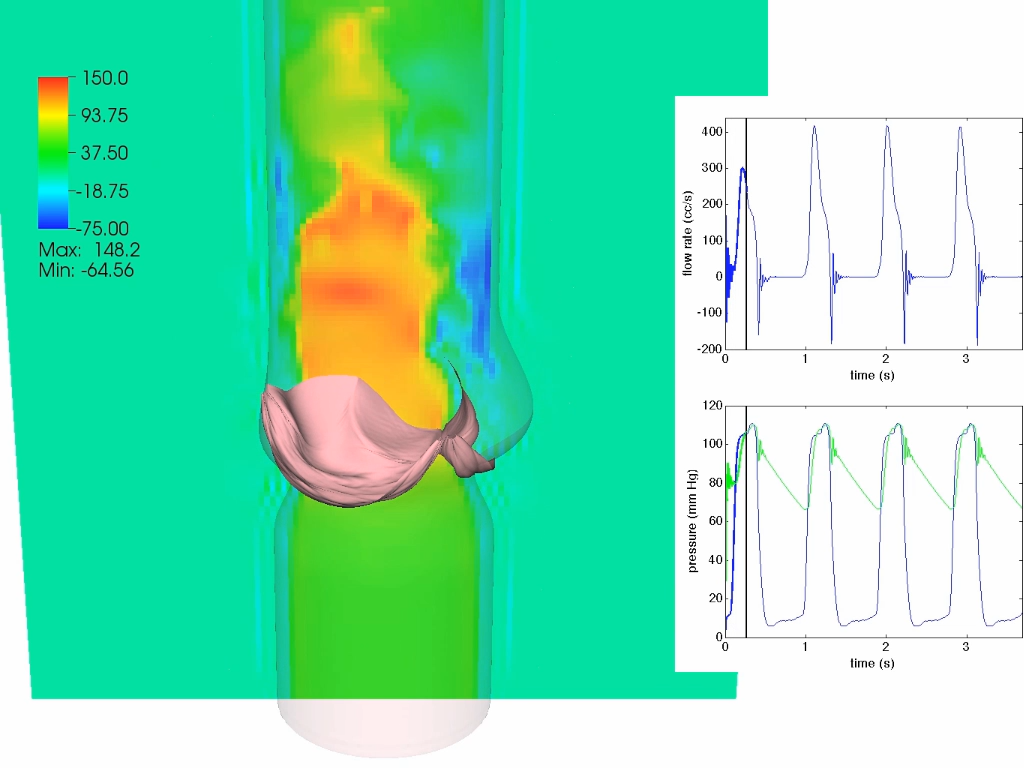
\includegraphics[width=9cm]{immersed_boundary/shot0002.png}
    \end{center}
\end{frame}

\begin{frame}
\frametitle{Аортальный клапан}
    \begin{center}
        \href{run:video/valve\_top.mov}{Демонстрация движения клапана}
    \end{center}
\end{frame}

\begin{frame}
\frametitle{Аортальный клапан}
    \begin{center}
        \href{run:video/valve\_flow\_side.mov}{Демонстрация течения жидкости}
    \end{center}
\end{frame}

%examples: mitral valve
\begin{frame}
\frametitle{Митральный клапан (протез)}
    \begin{center}
    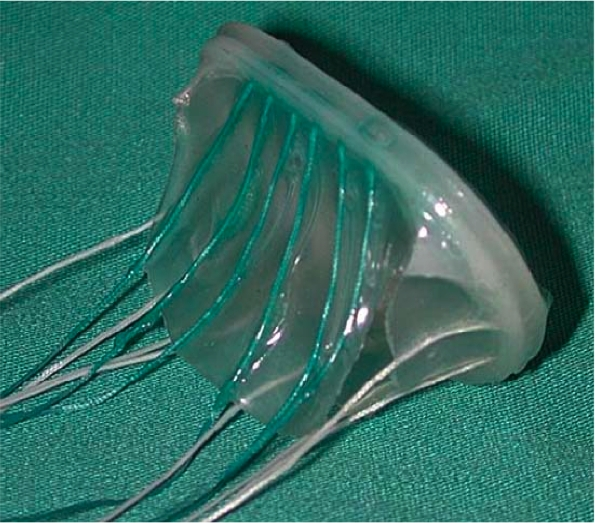
\includegraphics[width=8cm]{immersed_boundary/prosthetic_MV.jpeg}
    \end{center}
\end{frame}

\begin{frame}
\frametitle{Митральный клапан (протез)}
    \begin{center}
    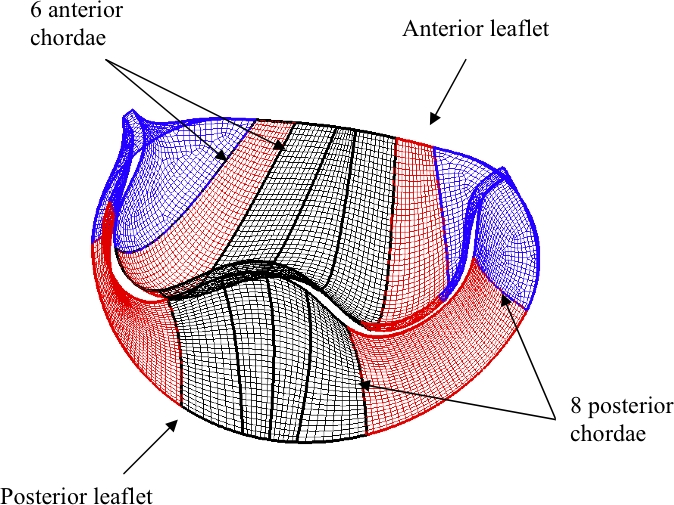
\includegraphics[width=9cm]{immersed_boundary/MV_mesh.jpeg}
    \end{center}
\end{frame}

\begin{frame}
\frametitle{Митральный клапан (линии тока)}
    \begin{center}
    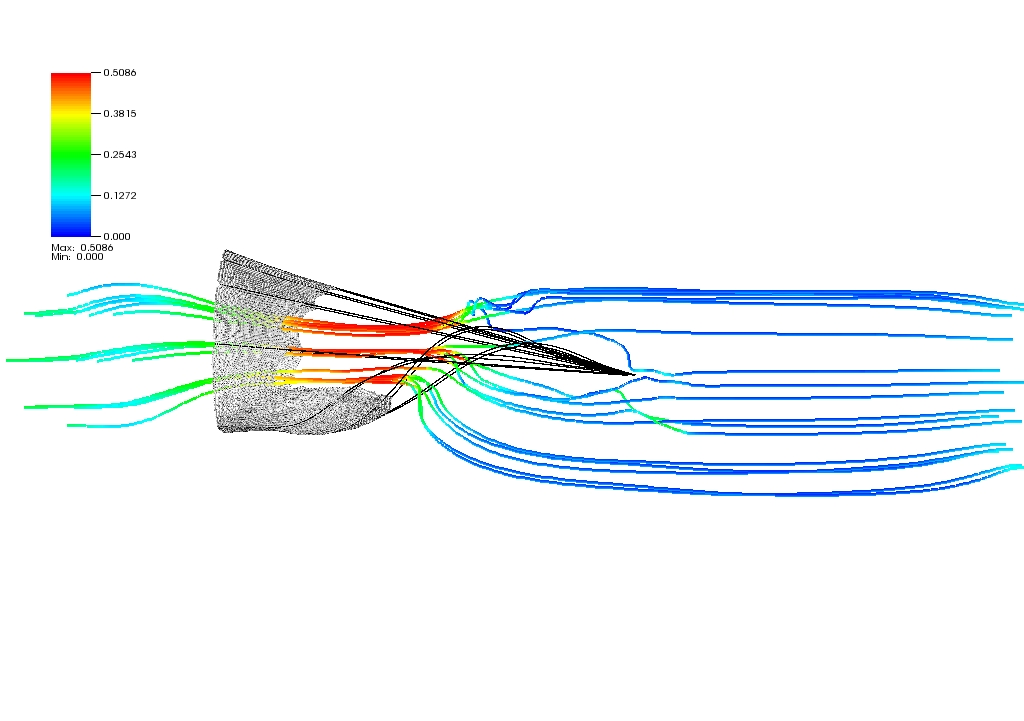
\includegraphics[width=9cm]{immersed_boundary/MV_streamline_0030.jpeg}
    \end{center}
\end{frame}

\begin{frame}
\frametitle{Митральный клапан}
    \begin{center}
        \href{run:video/MV\_side.mov}{Демонстрация движения клапана}
    \end{center}
\end{frame}

\begin{frame}
\frametitle{Без согласования}
    \begin{center}
    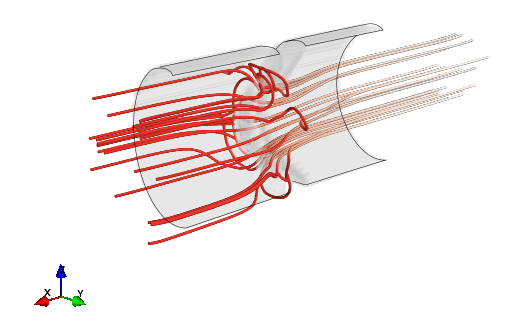
\includegraphics[width=9cm]{images/valves_resized_with_bound.png}
    \end{center}
\end{frame}

\begin{frame}
\frametitle{Без согласования}
    \begin{center}
    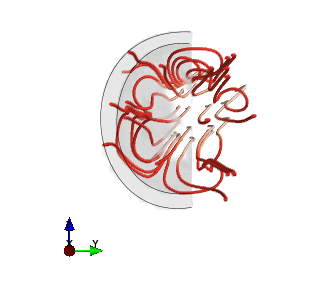
\includegraphics[width=9cm]{images/valves_resized_with_bound_front.png}
    \end{center}
\end{frame}

\begin{frame}
\frametitle{С согласованием}
    \begin{center}
    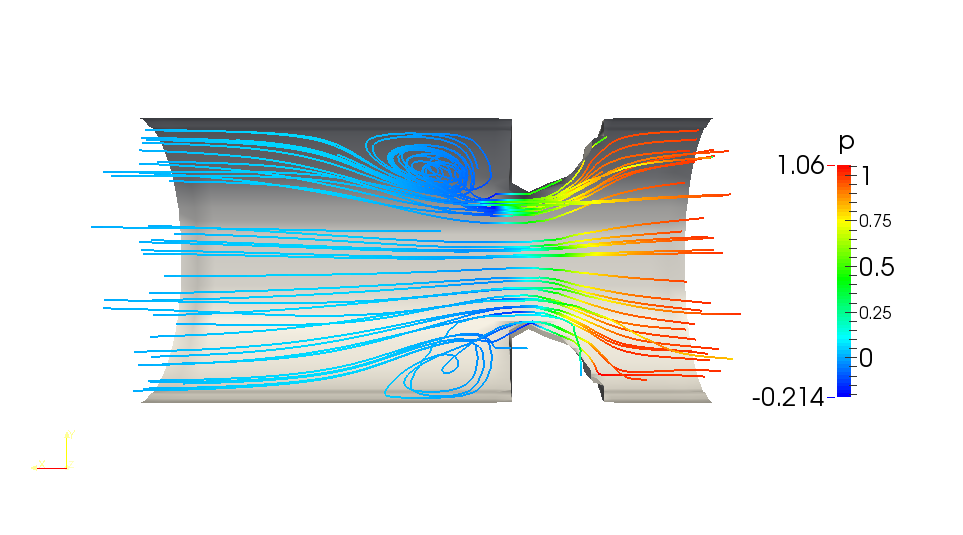
\includegraphics[width=9cm]{images/valves_simple.png}
    \end{center}
\end{frame}

\begin{frame}
\frametitle{С согласованием}
    \begin{center}
    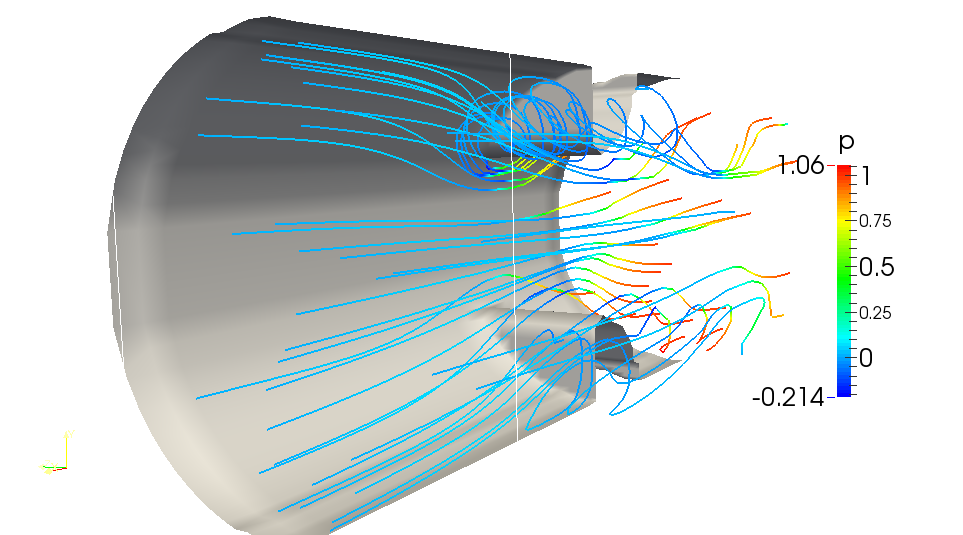
\includegraphics[width=9cm]{images/valves_simple_angle.png}
    \end{center}
\end{frame}

\begin{frame}
\frametitle{Обтекание сферы}
    \begin{center}
    \includegraphics[width=10cm]{images/ibm_results/correct/low_viscosity3_1_crop.png}
    \end{center}
\end{frame}

\begin{frame}
\frametitle{Обтекание сферы}
    \begin{center}
    \includegraphics[width=10cm]{images/ibm_results/correct/low_viscosity3_2_crop.png}
    \end{center}
\end{frame}

\begin{frame}
\frametitle{Обтекание сферы}
    \begin{center}
    \includegraphics[width=10cm]{images/ibm_results/correct/low_viscosity2_crop.png}
    \end{center}
\end{frame}

\begin{frame}
\frametitle{Дополнительная информация}
    \begin{itemize}
        \item Peskin C.S., Numerical Analysis of Blood Flow in the Heart// JCP 25,220-252, (1977)
        \item Peskin C.S., The immersed boundary method, (1977)
        \item Mittal R, Iaccarino G, Immersed boundary method// ARFM, 37, 239-261, (2005)
        \item Bandringa H., Immersed boundary method, Groningen, (2010)
    \end{itemize}
\end{frame}
\note{
    \begin{itemize}
        \item Основная работа "непрерывного метода" (journal of computational physic)
        \item Более полная и развернутая
        \item Хороший обзор (Annual Review of Fluid Mechanics)
        \item Обзор в диссертационной работе
    \end{itemize}
}

\begin{frame}
\frametitle{Дополнительная информация}
    \begin{itemize}
        \item Kruger T., Introduction to the immersed boundary method, (2011)
        \item Mital R., Seo J.H., A sharp-interface immersed boundary method with improved mass conservation and reduced spurious pressure oscillations// JCP, 230,7347-7363, (2011)
        \item Ghias R., Mital R., Dong H., A sharp interface immersed boundary method for compressible viscous flows// JCP, 225,528-553, (2007)
    \end{itemize}
\end{frame}
\note{
    \begin{itemize}
        \item Больше практики, но со спецификой другого метода расчета (Lattice Boltzmann method - метод решеточных уравнений Больцмана)
        \item О "дискретном"
        \item О "дискретном"
    \end{itemize}
}


\end{document}
